55. $\cfrac{4}{x^2-x-6}\geqslant(2+x)^{-1}\Leftrightarrow\cfrac{4}{(x-3)(x+2)}-\cfrac{1}{x+2}\geqslant0\Leftrightarrow\cfrac{4-x+3}{(x-3)(x+2)}\geqslant0
\Leftrightarrow\cfrac{7-x}{(x-3)(x+2)}\geqslant0.$ Применив метод интервалов, найдём ответ: $x\in(-\infty;-2)\cup(3;7].$
\begin{figure}[ht!]
\center{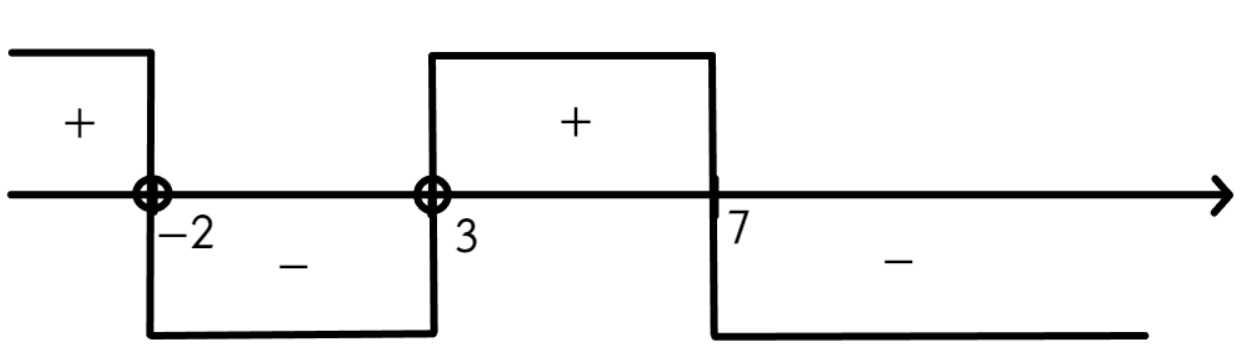
\includegraphics[scale=0.35]{ner9-55.png}}
\end{figure}\\
